%!TEX root=../GaugeCNNTheory.tex


\subsection{کلاف مماس \lr{\textit{TM}} و کلاف چارچوب \lr{\textit{FM}}}
\label{sec:GL_associated_bundles}


هر خمینه دیفرانسیل‌پذیر (و بنابراین هر خمینه ریمانی) $M$ به طور کانونی به کلاف مماس خود $\TM$ و کلاف چارچوب (عام) $\FM$ مجهز است، که از تمام چارچوب‌های مرجع محلی فضاهای مماس تشکیل شده است.
این دو کلاف به طور طبیعی به یکدیگر وابسته‌اند و گروه ساختار آنها به طور پیشینی توسط $\Aut(\R^d) = \GL{d}$ داده می‌شود.
این واقعیت با "بازسازی" $\TM$ از $\FM$ از طریق یک ساختار کلاف وابسته تأکید خواهد شد که بعداً به ما امکان می‌دهد کلاف‌های برداری ویژگی وابسته را تعریف کنیم.
برای جدا کردن واضح مفاهیم معرفی شده و فرضیات انجام شده، ما در اینجا $\TM$ و $\FM$ را به عنوان کلاف‌های $\GL{d}$ توصیف خواهیم کرد.
بخش بعدی~\ref{sec:G_associated_bundles} علاوه بر این یک $G$-ساختار را بر $\TM$ و $\FM$ تحمیل خواهد کرد که آنها را به عنوان $G$-کلاف‌ها تثبیت می‌کند.
در حالی که کلاف‌ها طبق تعریف به صورت محلی بدیهی‌شدنی هستند، ما در حال حاضر بدیهی‌سازی‌های خاص را مسلم فرض می‌کنیم و تعریف دقیق آنها را به بخش~\ref{sec:bundle_trivializations} موکول می‌کنیم.


\paragraph{کلاف مماس \lr{\textit{TM}}:}

هر خمینه هموار $M$ با مجموعه‌ای از فضاهای مماس $\TpM\cong\R^d$ همراه است.
اجتماع مجزای آنها%
\footnote{%
	اجتماع مجزای $\coprod_{p\in M} \TpM = \bigcup_{p\in M} \left\{(p,v) \,|\, v\in \TpM\right\}$ از فضاهای مماس را می‌توان به گونه‌ای تصور کرد که "به یاد می‌آورد" یک بردار خاص $v\in \TM$ از کدام فضای مماس خاص $\TpM$ سرچشمه می‌گیرد، که برای تعریف نگاشت تصویر $\piTM$ ضروری است.
}
\begin{align}
	\TM\ :=\, \coprod_{p\in M} \TpM \,,
\end{align}
به همراه یک ساختار هموار و نگاشت تصویر داده شده به طور کانونی، یک کلاف تاری هموار را تعریف می‌کند که به عنوان \emph{کلاف مماس} شناخته می‌شود.
نگاشت تصویر ${\piTM: \TM\to M}$ در این صورت با انتخاب بدیهی ${\piTM(v)=p}$ برای $v\in \TpM$ داده می‌شود.
همانطور که در پیوست~\ref{apx:coordinate_bases} استنتاج شده است، بدیهی‌سازی‌های محلی $\PsiTM: \piTM^{-1}(U) \to U\times \R^d$ از کلاف مماس به طور کانونی توسط چارت‌های $x:U\to V\subseteq \R^d$ از خمینه القا می‌شوند.
بنابراین می‌توانیم بدیهی‌شدنی بودن $\TM$ را مسلم فرض کرده و بحث در مورد آنها را به بخش~\ref{sec:bundle_trivializations} موکول کنیم.
یک ساختار هموار روی $\TM$ از ساختار هموار $M$ از طریق بدیهی‌سازی‌های فوق‌الذکر از چارت‌ها القا می‌شود.
ما از جزئیات فنی این ساختار صرف نظر کرده و خواننده علاقه‌مند را به مراجع~\cite{schullerGeometricalAnatomy2016,nakahara2003geometry} ارجاع می‌دهیم.

کلاف مماس تعریف شده بدین ترتیب یک \emph{کلاف برداری} است زیرا تار نوعی آن $\R^d$ یک فضای برداری است.
میدان‌های برداری مماس، که به عنوان مثال یک جریان روی $M$ را توصیف می‌کنند، به عنوان برش‌های $\sigma: M\to \TM$ از کلاف مماس فرمول‌بندی می‌شوند.
برش‌های سراسری هموار از کلاف‌های برداری همیشه وجود دارند؛ یک مثال استاندارد برش صفر است که بردار صفر از $\TpM$ را به هر $p\in M$ نسبت می‌دهد.
می‌خواهیم تأکید کنیم که فضاهای مماس -- و بنابراین کلاف مماس -- بدون ارجاع به چارچوب‌های مختصاتی تعریف می‌شوند، به طوری که برش‌ها میدان‌های برداری را به روشی مستقل از مختصات توصیف می‌کنند.

پس از معرفی کلاف چارچوب مماس $\FM$ در ادامه، به کلاف مماس و ساختار صریح آن به عنوان کلاف $\GL{d}$-وابسته باز خواهیم گشت که بر ماهیت مستقل از مختصات آن تأکید می‌کند.
در بخش~\ref{sec:G_associated_bundles} ما به طور مشابه $\TM$ را به عنوان یک $G$-کلاف وابسته به یک $G$-ساختار $\GM$ خواهیم ساخت.


\begin{figure}
	\centering
	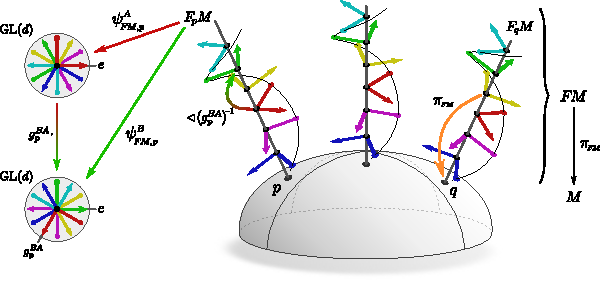
\includegraphics[width=1.\columnwidth]{figures/frame_bundle.pdf}
	\vspace*{-1ex}
	\caption{\small
		تفسیری گرافیکی از کلاف چارچوب $\FM$ روی~$M$ و بدیهی‌سازی‌های آن.
		تار~$\FpM$ روی~$p$ به عنوان فضای تمام چارچوب‌های مرجع ممکن~$\TpM$ تعریف می‌شود.
		تمام چارچوب‌ها در $\FpM$ توسط نگاشت تصویر $\piFM$ به همان نقطه $p$ در $M$ نگاشته می‌شوند که تار به آن متصل است.
		تارهای $\FpM$ با $\GL{d}$ یکریخت هستند، اما بدون مبدأی ارائه می‌شوند که یک انتخاب مرجح از چارچوب مرجع را متمایز کند.
		پیمانه‌های $\psiFMp^A: \FpM \to \GL{d}$ یا $\psiFMp^B: \FpM \to \GL{d}$ که در بخش~\ref{sec:bundle_trivializations} در ادامه معرفی می‌شوند، تارها را با $\GL{d}$ یکی می‌دانند و در نتیجه یک چارچوب مرجح را مشخص می‌کنند.
		پیمانه‌های مختلف با تبدیلات پیمانه $g_p^{BA} \in \GL{d}$ به هم مرتبط هستند.
		باید خواننده را در مورد دو تصور غلط احتمالی هشدار دهیم:
		اولاً، چارچوب‌ها در تارهای مختلف به طور پیشینی به روشی کانونی با یکدیگر یکی دانسته نمی‌شوند، چیزی که ممکن است رنگ‌های اضافی نشان دهند.
		ثانیاً، برای به حداقل رساندن شلوغی، تصویر فقط چارچوب‌های راست‌گرد و متعامد را به جای تمام چارچوب‌های مرجع ممکن نشان می‌دهد.
		همانطور که در بخش بعدی~\ref{sec:G_associated_bundles} بحث خواهیم کرد، چارچوب‌های متعامد و راست‌گرد نشان داده شده، متناظر با یک $G$-ساختار $\GM$ (یک زیرکلاف اصلی $G$ از $\FM$) برای گروه ساختار $G=\SO2$ خواهند بود.
	}
	\label{fig:frame_bundle}
\end{figure}

\paragraph{کلاف چارچوب \lr{\textit{FM}}:}
فضای چارچوب‌های مرجع محلی تمام فضاهای مماس $\TpM$ ، (کلاف) \emph{چارچوب} (مماس) را تشکیل می‌دهد.
فضاهای چارچوب‌های مرجع (پایه‌های مرتب) فضاهای مماس منفرد $\TpM$ را در نظر بگیرید:
\begin{align}
	\FpM\ :=\ \pig\{ \big[e_{1},\dots,e_{d}\big]\, \pig|\ \{e_{1},\dots,e_{d}\}\ \text{یک پایه از } \TpM \text{ است} \pig\}
\end{align}
کلاف چارچوب به عنوان اجتماع مجزای آنها $\FM := \coprod_{p\in M} \FpM$ به همراه نگاشت تصویر $\piFM: \FM\to M$ که چارچوب‌ها در $\FpM$ را به $p$ می‌فرستد و یک ساختار هموار القا شده از $\TM$ تعریف می‌شود.
تار نوعی کلاف چارچوب، گروه خطی عام $\GL{d}\cong \FpM$ است، یعنی گروه ماتریس‌های معکوس‌پذیر $d\!\times\!d$ که ستون‌های مستقل خطی آن را می‌توان به عنوان تعریف‌کننده یک چارچوب از $\R^d$ در نظر گرفت.
از آنجا که کلاف چارچوب از کلاف مماس ساخته شده است، بدیهی‌سازی‌های محلی آن $\PsiFM: \piFM^{-1}(U) \to U \times \GL{d}$ بلافاصله از بدیهی‌سازی‌های $\TM$ القا می‌شوند؛ به بخش~\ref{sec:bundle_trivializations} مراجعه کنید.
شکل~\ref{fig:frame_bundle} تفسیری گرافیکی از کلاف چارچوب را نشان می‌دهد.


برش‌های هموار محلی $\sigma:U\to\piFM^{-1}(U)\subseteq \FM$ از کلاف چارچوب، نقاط $p\in U$ را به چارچوب‌هایی در $\FpM$ نگاشت می‌کنند.
آنها میدان‌های چارچوب هموار محلی را تعریف می‌کنند، یعنی انتخاب‌های هموار متغیر از چارچوب‌های مرجع برای $\TpM,\ p\in U$؛ که در شکل~\ref{fig:gauge_trafos_manifold} به تصویر کشیده شده است.
همانطور که در معادله~\eqref{eq:framefield_gauge_equivalence} استدلال شد، یک انتخاب از میدان چارچوب روی $U$ با یک انتخاب از پیمانه یا بدیهی‌سازی محلی روی $U$ \emph{معادل} است.
این ایجاب می‌کند که میدان‌های چارچوب سراسری تنها در صورتی وجود داشته باشند که $\FM$ -- و در نتیجه $\TM$ -- بدیهی باشند.
ما این هم‌ارزی را با عمق بیشتری در بخش~\ref{sec:bundle_trivializations} مورد بحث قرار خواهیم داد.

یک عمل راست تعدی‌پذیر و آزاد بر روی تارهای منفرد $\FpM\cong\GL{d}$ از کلاف چارچوب به طور طبیعی توسط تغییر چارچوب‌ها که در معادله~\eqref{eq:frame_rightaction} تعریف شده است، داده می‌شود~\cite{schullerGeometricalAnatomy2016}.
عمل متناظر
\begin{align}\label{eq:rightaction_FM}
	\lhd:\ \FM\times \GL{d} \to \FM, \quad
	\big( [e_i]_{i=1}^d,\ g \big)
	\ \mapsto\ 
	[e_i]_{i=1}^d\! \lhd g \ :=\ 
	\left[ \sum\nolimits_j e_j\, g_{ji} \right]_{i=1}^d
\end{align}
روی $\FM$ به عنوان یک کل، کلاف چارچوب را به یک کلاف اصلی $\GL{d}$ تبدیل می‌کند.
فقدان مبدأ یا عنصر همانی مرجح در تارهای $\FpM$ به عنوان $\GL{d}$-تورسورها، ابهام ذاتی چارچوب‌های مرجع را منعکس می‌کند.


\paragraph{کلاف \lr{\textit{TM}} به عنوان کلاف برداری وابسته به \lr{GL(\textit{d})} ($(\FM\times \mathds{R}^d)/$ \lr{GL(\textit{d})}):}
در بخش~\ref{sec:gauges_gauge_trafos} ما بردارهای مماس در $\TpM$ را بر حسب ضرایب آنها در $\R^d$ نسبت به یک چارچوب مرجع بیان کردیم.
انتخاب خاص چارچوب‌ها در آنجا بی‌ربط بود زیرا تبدیل ضرایب در معادله~\eqref{eq:components_leftaction} با تبدیل چارچوب‌های مرجع در معادله~\eqref{eq:frame_rightaction} خنثی می‌شود به طوری که $v = \sum_i v^A_i e^A_{i} = \sum_i v^B_i e^B_{i}$ نمایش‌های مختصاتی معادل از همان بردار مستقل از مختصات $v\in \TpM$ هستند.
با پیروی از این ایده، می‌توان کلاف مماس را از کلاف چارچوب با جفت کردن چارچوب‌های مرجع با بردارهای ضریب و گرفتن یک خارج‌قسمت برای فروکاستن توصیفات اضافی حاصل از بردارهای مماس نسبت به چارچوب‌های مختلف به یک عنصر منحصربه‌فرد، ساخت.

برای ساختن کلاف مماس به این روش، حاصلضرب $\FM\times\R^d$ را در نظر بگیرید که می‌توان آن را به عنوان یک کلاف تاری با فضای پایه $M$ و یک تار نوعی $\GL{d}\times\R^d$ دید.
این کلاف از جفت‌های چارچوب‌های مرجع و ضرایب (متقابلاً نامرتبط) تشکیل شده است.
با انگیزه از بیان معادل بردارهای مماس در چارچوب‌های مرجع مختلف، ما \emph{رابطه هم‌ارزی} را تعریف می‌کنیم:%
\footnote{\label{footnote:equiv_rel}%
	یک \emph{رابطه هم‌ارزی} روی یک مجموعه $X$ یک رابطه دوتایی $\sim$ است که
	\emph{بازتابی} ($x\!\sim\! x$)،
	\emph{متقارن} ($x\!\sim\! y \Leftrightarrow y\!\sim\! x$) و
	\emph{تراگذری} ($x\!\sim\! y \wedge y\!\sim\! z \Rightarrow x\!\sim\! z$) است.
	این رابطه یک افراز از $X$ به \emph{کلاس‌های هم‌ارزی} $[x] := \{y\in X | x\sim y\}$ از عناصر $x\in X$ تعریف می‌کند.
	فضای کلاس‌های هم‌ارزی $X/\!\!\sim\ := \{[x] \,|\, x\in X\}$ را \emph{مجموعه خارج‌قسمتی} $X$ بر $\sim$ می‌نامند.
}
\begin{align}\label{eq:equiv_relation_TM}
	\big([e_i]_{i=1}^d,\,\mathscr{v}\big)\ \sim_{\GL{d}}\, \big([e_i]_{i=1}^d\!\lhd g^{-1},\, g\cdot \mathscr{v}\big) \qquad\forall\, g\in \GL{d}
\end{align}
روی $\FM\times\R^d$.
به عنوان یک رابطه هم‌ارزی، این رابطه $\FM\times\R^d$ را به \emph{کلاس‌های هم‌ارزی} $\big[[e_i]_{i=1}^d,\,\mathscr{v}\big]$ افراز می‌کند.
فضای این کلاس‌های هم‌ارزی، فضای خارج‌قسمتی $(\FM\times\R^d)/\GL{d}$ است.
نگاشت تصویر
\begin{align}\label{eq:associated_TM_proj}
	\pi_{\scalebox{.75}{$\sim_{\GL{d}}$}}:\ 
	(\FM\times\R^d)/\GL{d} \to M,\ \ 
	\big[[e_i]_{i=1}^d,\,\mathscr{v}\big] \mapsto \piFM\!\left([e_i]_{i=1}^d\right) \,,
\end{align}
که از کلاف چارچوب القا شده است، $(\FM\times\R^d)/\GL{d}$ را به یک کلاف تاری با فضای پایه $M$ و تار نوعی~$\R^d$ تبدیل می‌کند.
توجه داشته باشید که نگاشت تصویر در معادله~\eqref{eq:associated_TM_proj} خوش‌تعریف است زیرا مستقل از نماینده کلاس هم‌ارزی است، یعنی
$\pi_{\scalebox{.75}{$\sim_{\GL{d}}$}}\left(\big[[e_i]_{i=1}^d\lhd g^{-1},\, g\cdot \mathscr{v}\big]\right) := \piFM\left([e_i]_{i=1}^d\!\lhd g^{-1}\right) = \piFM\left([e_i]_{i=1}^d\right)$،
که در آن ما از این واقعیت استفاده کردیم که عمل راست $\lhd$ تارهای $\FM$ را حفظ می‌کند.
ساختار فضای برداری $\R^d$ ، $(\FM\times\R^d)/\GL{d}$ را به یک کلاف برداری تبدیل می‌کند که ترکیبات خطی در همان تار توسط
\begin{align}\label{eq:associated_bdl_linear_combination}
	\alpha \big[[e_i]_{i=1}^d,\,\mathscr{v}\big] + \beta \big[[e_i]_{i=1}^d,\,\mathscr{w}\big]
	\ :=\ \big[[e_i]_{i=1}^d,\,\alpha\mathscr{v} + \beta\mathscr{w} \big] \,,
\end{align}
برای مقادیر دلخواه $\alpha,\beta\in\R$ و $\mathscr{v},\mathscr{w}\in\R^d$ تعریف می‌شود.
به راحتی می‌توان بررسی کرد که این تعریف مستقل از انتخاب نماینده در هر دو جمله جمع است.

کلاف تعریف شده بدین ترتیب با کلاف مماس یکریخت است،
\begin{align}
	\TM\, \cong\, (\FM\times\R^d)/\GL{d} \,,
\end{align}
که در آن یکریختی $M$-کلاف برداری توسط نگاشت خطی به ازای هر تار
\begin{align}\label{eq:A_TM_isomorphism}
	\chi:(\FM\times\R^d)/\GL{d}\ \to \TM,\ \ \ \left[[e_i]_{i=1}^d,\, \mathscr{v}\right] \mapsto \sum_{i=1}^d \mathscr{v}_i e_i
\end{align}
داده می‌شود که یک تاپل نماینده از چارچوب و بردار ضریب را از کلاس هم‌ارزی گرفته و آنها را به بردار مماس متناظر نگاشت می‌کند.
طبق تعریف رابطه هم‌ارزی $\sim_{\GL{d}}$، این تابع مستقل از انتخاب نماینده است، یعنی،
$
\forall g\in \GL{d}: \ 
\chi\left( \big([e_i]_{i=1}^d\lhd g^{-1},\, g\cdot \mathscr{v}\big) \right) = 
{\sum_i (g\!\cdot\!\mathscr{v})_i \left([e_j]_{j=1}^d\!\lhd g^{-1}\right)_i} =
\sum_i \mathscr{v}_i e_i \, ;\,
$
مقایسه کنید با معادله~\eqref{eq:vector_in_different_bases}.
همانطور که در~\cite{schullerGeometricalAnatomy2016} بحث شد، معکوس این نگاشت با گرفتن یک بردار مماس، تصویر کردن آن بر روی یک چارچوب دلخواه و گرفتن کلاس هم‌ارزی به دست می‌آید.


کلاف $(\FM \times \R^d) / \GL{d}$ طبق ساختار، به $\FM$ به عنوان یک کلاف $\GL{d}$-وابسته، وابسته است، یعنی همان توابع گذار را در $\GL{d}$ دارد که $\FM$ دارد، همانطور که در بخش~\ref{sec:bundle_trivializations} استنتاج خواهیم کرد.
ساختار $\TM$ به عنوان خارج‌قسمت $(\FM\times\R^d)/\GL{d}$ بر ماهیت \emph{مستقل از مختصات} کلاف مماس به روشی بسیار شهودی تأکید می‌کند:
این ساختار تمام انتخاب‌های ممکن از مختصات‌دهی‌های فضاهای مماس را در نظر گرفته و با گرفتن یک خارج‌قسمت، آنها را معادل تلقی می‌کند.